\documentclass{beamer}

%%%%%%%%%%%%%%%%%%%% Package declarations %%%%%%%%%%%%%%%%

%\usepackage[utf8]{inputenc}
\usepackage[brazil]{babel}
\usepackage{graphics}
\usepackage{graphicx} 
\usepackage{mathptmx}
\usepackage[scaled=.90]{helvet}
\usepackage{courier}
\usepackage{listings}
\usepackage{tikz}
\usepackage[T1]{fontenc}
\usepackage{bussproofs}

\mode<presentation>
{
\usetheme{Boadilla}

\setbeamercovered{transparent}
}
\setbeamertemplate{navigation symbols}{} 
\setbeamertemplate{frametitle}
{
\vspace{0.5cm}\LARGE\insertframetitle\par
}

\usetikzlibrary{decorations.pathmorphing} % noisy shapes
\usetikzlibrary{fit}					% fitting shapes to coordinates
\usetikzlibrary{backgrounds}	% drawing the background after the foreground
\usetikzlibrary{positioning}

\definecolor{listinggray}{gray}{0.9}
\lstset{
	tabsize=2,
	numbers=left,
	numbersep=5pt,
	xleftmargin=15pt,
	framexleftmargin=15pt,
	rulecolor=,
	numberstyle=\scriptsize,
	captionpos=b,
	mathescape=true,
        basicstyle=\footnotesize,
        columns=fixed,
        basewidth=0.54em,
        showstringspaces=false,
        extendedchars=true,
        breaklines=true,
        prebreak = \raisebox{0ex}[0ex][0ex]{\ensuremath{\hookleftarrow}},
        frame=none,
        showtabs=false,
        showspaces=false,
        showstringspaces=false,
        identifierstyle=\ttfamily,
        keywordstyle=\color[rgb]{0,0,1},
        commentstyle=\color[rgb]{0.133,0.545,0.133},
        stringstyle=\color[rgb]{0.627,0.126,0.941},
}

%%%%%%%%%%%%%%%%%%%% New commands declarations %%%%%%%%%%%%
\newcommand{\putat}[3]{\begin{picture}(0,0)(0,0)\put(#1,#2){#3}\end{picture}}

\title[Projetos de Pesquisa]{Grupo de Pesquisa em Linguagens de Programa\c c\~ao, Verifica\c c\~ao e Engenharia de Sistemas}

\author[Lives]{Elton M\'aximo \\ Glauber Cabral \\ Leonardo Reis \\ Rodrigo Ribeiro}


\institute[]{
Departamento de Computa\c c\~ao e Sistemas (DECSI)
}

\date{18 de Junho, 2015}

\subject{Talks}

\begin{document}

\begin{frame}
%\putat{-11}{-55}{
\includegraphics[width=12.8cm]{img/logo}}
%\newline \newline \newline
\titlepage
\end{frame}

\begin{frame}[t]
  \frametitle{Projetos}
  \tableofcontents %[pausesections]
\end{frame}

\section{Rodrigo'work}

\begin{frame}
 \frametitle{Espa�o do Rodrigo}
\end{frame}

\section{Modulariza��oo e Extensibilidade de Linguagens}

\begin{frame}
  \frametitle{Era da Produtividade}
%  \putat{200}{-10}{
\includegraphics[width=3.8cm]{img/efficiency_01}}
  \putat{200}{-10}{
\includegraphics[width=3.6cm]{img/focus}}
  \begin{itemize}
    \item Foco na efici�ncia do programador
    \item DSLs como uma alternativa para melhorar a efici�ncia do programador
    \item Linguagens extens�veis como mecanismo para implementar e usar DSLs
  \end{itemize}
  \putat{5}{-70}{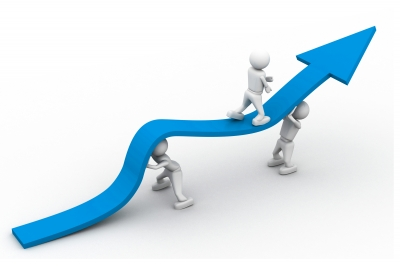
\includegraphics[width=3.5cm]{img/efficiency}}
\end{frame}

\begin{frame}[fragile]
  \frametitle{O que s�o Linguagens Extens�veis?}
  \begin{itemize}
    \item Linguagens extens�veis s�o linguagens que permitem estender a pr�pria sintaxe concreta
  \end{itemize}
    \begin{columns}[!ht]
    \begin{column}{5.5cm}
\begin{lstlisting}[language=java,
                   frame=bottomline,title={SugarJ defining syntax}]
package syntactic;
public sugar Pair {
  context-free syntax
   "("JavaType "," JavaType")" 
        $\rightarrow$ $\alert<1>{JavaType}$
   "("JavaExpr "," JavaExpr")" 
        $\rightarrow$ $\alert<2>{JavaExpr}$
  ...
}
\end{lstlisting}
    \end{column}
    \begin{column}{5.5cm}
\begin{lstlisting}[language=java,frame=bottomline,title={Using Pair syntax},escapechar=\%]
import syntactic.Pair;
public class Test {
 private $\alert<1>{(String, Integer)}$ p 
               = %\alert<2>{("12", 34)}%;
}
\end{lstlisting}
    \end{column}
  \end{columns}
\end{frame}

\defverbatim[colored]\sugarj{
    \begin{columns}[!ht]
    \begin{column}{5.5cm}
\begin{lstlisting}[language=java,
                   frame=bottomline,title={SugarJ defining syntax}]
package syntactic;
public sugar Pair {
  context-free syntax
   "("JavaType "," JavaType")" 
        $\rightarrow$ JavaType
   "("JavaExpr "," JavaExpr")" 
        $\rightarrow$ JavaExpr
  ...
}
\end{lstlisting}
    \end{column}
    \begin{column}{5.5cm}
\begin{lstlisting}[language=java,frame=bottomline,title={Using Pair syntax},escapechar=\%]
%\alert{import syntactic.Pair;}%
public class Test {
 private (String, Integer) p 
               = ("12", 34);
}
\end{lstlisting}
    \end{column}
  \end{columns}
}

\begin{frame}[fragile]
  \frametitle{Como Essas Caracter�sticas Din�micas Afetam o Parsing?}
  \begin{itemize}
    \item Necessidade de modificar o parser de forma din�mica, durante a an�lise da entrada
  \end{itemize}
  \sugarj
\end{frame}

\begin{frame}
  \frametitle{As Teorias de Parsing Suportam Modifica��o Din�mica?}
  \begin{itemize}
    \item Principais avan�os recentes na �rea n�o tratam de modifica��es din�micas
      \begin{itemize}
        \item PEG, LL(*), Adaptative LL(*), SGLR, YAKKER
      \end{itemize}
    \item Trabalhos que lidam com modifica��o din�mica das regras t�m efici�ncia question�vel ou n�o apresentam algoritmos de parsing
      \begin{itemize}
        \item Adaptable Grammar de Christiansen; RAG; Parsing Reflective Grammars;
        \item AMG; Dynamic Grammars; Evolving Grammars
      \end{itemize}
  \end{itemize}
  %\hspace{9cm} 
\includegraphics[width=2.5cm]{img/question.jpg}
  \putat{270}{-60}{
\includegraphics[width=2.5cm]{img/question.jpg}}
\end{frame}

\begin{frame}[fragile]
  \frametitle{Adaptable Parsing Expression Grammars}
  \begin{itemize}
   \item Extens�o de Parsing Expression Grammar;
   \item Modelo que permite modifica��es no conjunto de regras dinamicamente.
  \end{itemize}
  \putat{220}{45}{
\includegraphics[width=4cm]{img/efficiency_01}}
  \putat{10}{-100}{
\includegraphics[width=4cm]{img/camaleao}}
  \putat{220}{-90}{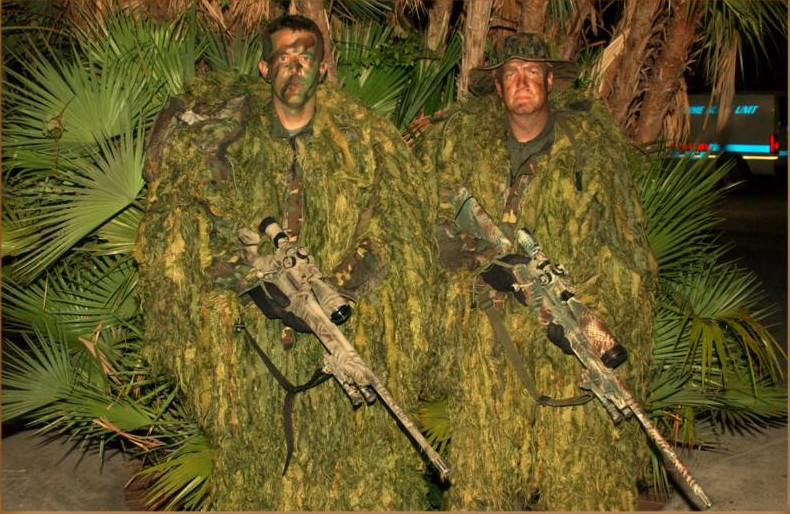
\includegraphics[width=4cm]{img/adapt}}
\end{frame}

\begin{frame}
 \frametitle{A Pesquisa}
 \begin{itemize}
  \item Desenvolvimento de um gerador autom�tico de analisador sint�tico baseado em APEG:
   \begin{itemize}
    \item Implementa��o eficiente;
    \item Tratamento de erros;
    \item Constru��o autom�tica de AST e metaprograma��o;
    \item provas de propriedades;
   \end{itemize}
  \item An�lise (m�trica) de uso de DSLs em sistema reais;
  \item Estudo de formalismos e mecanismo para especifica��o modular de linguagens
 \end{itemize}
\end{frame}

\section{Elton'work}

\begin{frame}
 \frametitle{Espa�o do Elton}
\end{frame}

\section{Glauber'work}

\begin{frame}
 \frametitle{Espa�o do Glauber}
\end{frame}

\end{document}
